We now show an example of discrete dynamics, used as a case study throughout this paper. Let us consider a game where a guard patrols a room. A set of enemies will periodically enter the room and try to walk through the guard post. The guard is given a set of waypoints which will form the patrol route. A healer will periodically visit the guard post to offer healing services.

The behaviour of the guard can be re-defined as a set of prioritized tasks, listed by descending priority, as follows:
\begin{enumerate}
\item Health $< 0 \Rightarrow$ The guard is dead.
\item Low health $\Rightarrow$
	\begin{enumerate}
		\item Enemy near $\Rightarrow$ retreat
		\item Healer available $\Rightarrow$ Go to the healer and recover.
		\item Otherwise $\Rightarrow$ Do nothing.
	\end{enumerate}
\item An enemy is in range $\Rightarrow$ Attack the enemy.
\item Otherwise $\Rightarrow$ cycle through waypoints and slowly recover health.
\end{enumerate}

These tasks can be modelled by the \textit{Behaviour Tree} shown in Figure \ref{fig:s2f1}. In this representation we used the notation $\emptyset$ for the root node of the tree, and ? for \textit{fallback nodes}. A fallback node will return immediately when the first of its children succeeds, ticking them from left to right.

\begin{figure}
	\centering
	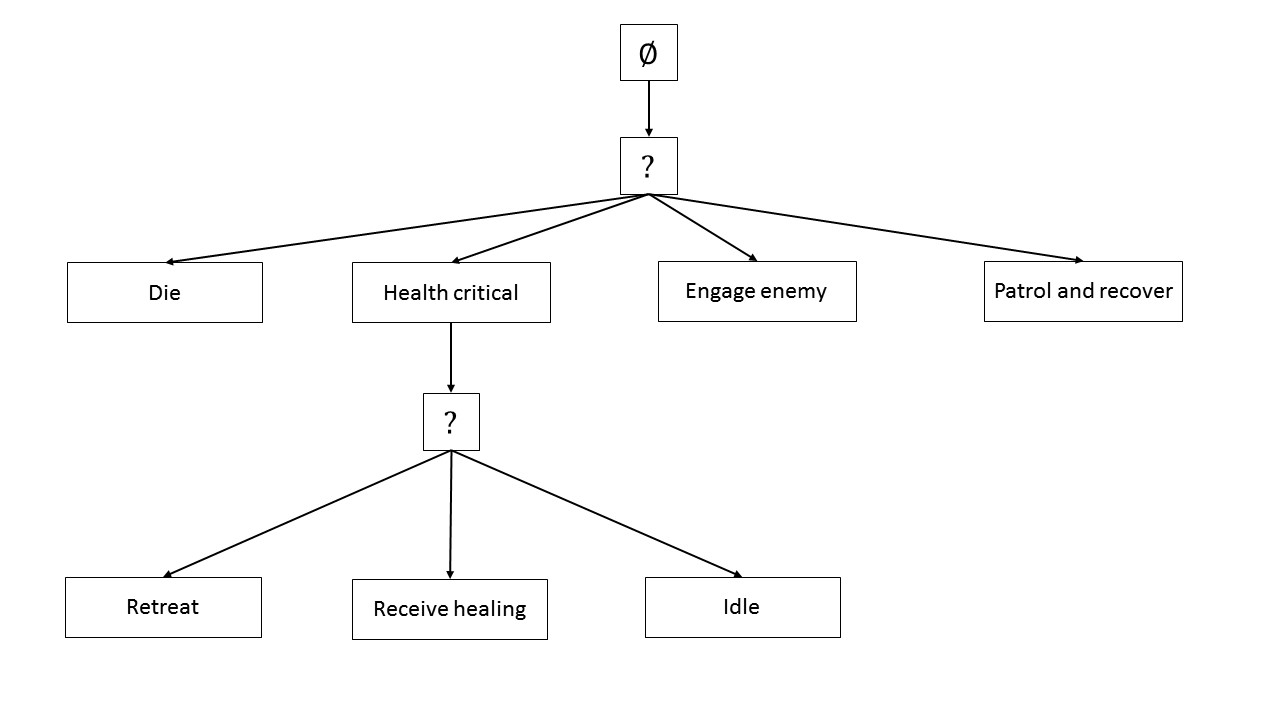
\includegraphics[scale=0.35]{Image/Behaviour_tree}
	\caption{Guard behaviour tree}
	\label{fig:s2f1}
\end{figure}
Note that, according to the priority rule defined above, if there is an enemy near the guard but his health is critical (i.e. below a specified threshold), he will run a retreat/heal subtask.

This example illustrates how even a simple behaviour, such as that of the guard, requires very complex control structures which must be implemented manually by the programmer. From the case study the following behavioural patterns emerge:

\begin{itemize}

\item \textit{Waiting}: used during the self-healing of the guard while patrolling, since the health must increase only after an interval of time has elapsed.

\item \textit{Concurrency}: used for choosing which task the guard must accomplish.

\item \textit{Parallelism}: used during the guard patrol, when he moves to the next waypoint and at the same time he recovers health periodically.

\item \textit{Pre-emption}: used to abort a task when another task with higher priority is ready to be executed.

\item \textit{Nesting}: used when building sub-tasks for the guard.
\end{itemize}

If these patterns are not well supported by a programming language, they must be rebuilt every time. This requires to manually manage the coordination between states, and increases the chance of errors in the code. Although derived from this case study, we argue that this operators are general enough to cover the most common discrete dynamics used in games, by combining them appropriately.

\vspace{0.5cm}
In the following section we will give a brief introduction to the Casanova 2 language, a declarative-imperative programming language oriented to the development of video games. In Section \ref{sec:idea}, as anticipated above, we will show the definition of a set of discrete dynamics operators (based on the patterns described in the case study) and then introduce an optimization technique called \textit{lazy waiting} to reduce the overhead due to the waiting behaviour of these operators.

